\subsection{Use cases}
	\begin{alltt}
\rm
Next, the use cases for the game will be presented. These use cases are made to illustrate how the game works and what possible scenarios can be occur. In the use cases, a trigger for the use case and a pre-condition for the use case can be found. After that, the main scenario (usual case) of the use case will be presented and after that possible alternatives can be found.

The "Initialize viewer" use case illustrates the Initialize viewer state in the High Level Message Sequence Chart. This use case is used to illustrate how the viewer will be initialized.

Initialize viewer
- Pre-conditions: True
- Trigger: World messages the viewer
- Guarantee: Initialized viewer
- Main Scenarios
    (a) Viewer initializes
    (b) Viewer sends a message to the controller that he is the viewer
- Alternatives

The "Update viewer" use case illustrates the Update viewer state in the High Level Message Sequence Chart. Use case for updating the viewer after something on the board has changed.

Update viewer
- Pre-conditions: The game is initiated
- Trigger: Notify and new snapshot by the controller
- Guarantee: Update viewer
- Main Scenarios
    (a) Update view by the received snapshot
- Alternatives

The next use case illustrates the initialize state in the High Level Message Sequence Chart. In this use case, all of the different components (except for the viewer) will get initialized.

Initialize
- Pre-conditions: True
- Trigger: The user presses the start game button.
- Guarantee: A new game is initiated.
- Main Scenarios
    (a) Initialize board
    (b) The board pre-initializes the controller
    (c) The board initializes all robots (one by one)
    (d) The board post-initializes the controller with all the robots
- Alternatives

The "Robot move request" use case illustrates the Robot move request state in the High Level Message Sequence Chart. In this use case, the robot request the controller if it can make a move. The controller forwards this request to the board, which then decides. Note that the board here checks if the move is allowed. This also deals with the fact that, if a robot wants to move to its home tile and this is occupied, the robot still may move (and moves) to this tile.

Robot move Request
- Pre-conditions: The game is initiated. And the indicated position
    is a empty tile.
- Trigger: A robot requests to move his position.
- Guarantee: The robot is moved to the indicated position.
- Main Scenarios
    (a) The robot requests the controller if it may move
    (b) The controller sends the request to the board
    (c) The board checks the request
- Alternatives


The "Return Normal tile" use case illustrates the Return Normal tile state in the High Level Message Sequence Chart. This use case always comes after the Robot move request use case. This use case handles with a robot for which his move request to go to a normal tile has been approved.

Return Normal tile
- Pre-conditions: The game is initiated. And the indicated position
    is a normal tile, move request approved.
- Trigger: A robot requests to move his position to a normal tile.
- Guarantee: The robot is moved to the indicated position which
    is a normal tile.
- Main Scenarios
    (a) The robot is moved to the indicated position which is a normal tile
    (b) The board notifies the controller that the move request has been approved
    (c) The controller notifies the robot that his move request has been approved and that the robot has been moved to the requested position
    (d) The board makes a snapshot and sends this to the controller
    (e) The controller notifies the viewer that there are changes and sends the snapshot along with this
- Alternatives


The "Return Hint tile" use case illustrates the Return Hint tile state in the High Level Message Sequence Chart. This use case always comes after the Robot move request use case. This use case handles with a robot for which his move request to go to a hint tile has been approved.

Return Hint tile
- Pre-conditions: The game is initiated. The indicated position
    is a hint tile, move request approved.
- Trigger: A robot requests to move his position to a hint tile.
- Guarantee: The robot is moved to the indicated position which
    is a hint tile and a hint is given to the player.
- Main Scenarios
    (a) The robot is moved to the indicated position which is a hint tile
    (b) The board notifies the controller that the move request has been approved
    (c) The controller notifies the robot that his move request has been approved and that the robot has been moved to the requested position
    (d) The board makes a snapshot and sends this to the controller
    (e) The controller notifies the viewer that there are changes and sends the snapshot along with this
    (f) The board generates a hint for the robot
    (g) The board notifies the controller of the hint and the robot it needs to be send to
    (h) The controller sends the hint to the robot
- Alternatives

The "Return Conveyor tile" use case illustrates the Return Conveyor tile state in the High Level Message Sequence Chart. This use case always comes after the Robot move request use case. This use case handles with a robot for which his move request to go to a conveyor tile has been approved.

Return Conveyor tile
- Pre-conditions: The game is initiated. And the indicated position
    is a conveyor tile, move request approved.
- Trigger: A robot requests to move his position to a conveyor
    belt tile.
- Guarantee: The robot is moved to the indicated position which
    is a conveyor belt tile.
- Main Scenarios
    (a) The robot is moved to the indicated position which is a conveyor
    (b) The board notifies the controller that the move request has been approved
    (c) The controller notifies the robot that his move request has been approved and that the robot has been moved to the requested position
    (d) The board calculates the new position (after movement over the conveyor tile)
    (e) The board makes a snapshot and sends this to the controller
    (f) The controller notifies the viewer that there are changes and sends the snapshot along
    (g) The board notifies the controller that a robot has been moved automatically
    (h) The controller notifies the robot that it has been moved automatically
- Alternatives

The "Return Home tile" use case illustrates the Return Home tile state in the High Level Message Sequence Chart. This use case always comes after the Robot move request use case. This use case handles with a robot for which his move request to go to his home tile has been approved.

Return Home tile
- Pre-conditions: The game is initiated. And the indicated position
    is its home tile, move request approved.
- Trigger: A robot requests to move his position to a home tile.
- Guarantee: The robot is moved to the indicated position which
    is its home tile.
- Main Scenarios
    (a) The robot is moved to the indicated position which is the robots home tile
    (b) The board notifies the controller that the move request has been approved and the robot has won
    (c) The controller notifies the robot that his move request has been approved, that the robot has been moved to the requested position and that the robot has won
    (d) The board makes a snapshot and sends this to the controller
    (e) The controller notifies the viewer that there are changes and sends the snapshot along
- Alternatives

The "Reject move" use case illustrates the Reject move state in the High Level Message Sequence Chart. This use case always comes after the Robot move request use case. This use case handles with a robot for which his move request has been rejected.

Reject move
- Pre-conditions: The game is initiated. A move request of a robot is rejected.
- Trigger: A robot requests to move
- Guarantee: The robot remains on the same position
- Main Scenarios
    (a) The board sends the reject message to the controller
    (b) The controller sends the reject message to the robot
- Alternatives

The "Tiles exchange" use case illustrates both the Special exchange and the Ordinary exchange state in the High Level Message Sequence Chart. In the "normal" case, two tiles are swapped (no robots on it and they are normal tiles). In the special cases, either a robot is on a tile and needs to be notified that its position has changed and he has been rotated. Or a conveyor belt is switched and rotated (or a combination of both).

Tiles exchange
- Pre-conditions: The game is initiated.
- Trigger:  A robot has moved.
- Guarantee: Two tiles are exchanged
- Main Scenarios
    (a) Two valid tiles are chosen
    (b) The chosen tiles are exchanged (ordinary exchange)
    (c) The board makes a snapshot and sends this to the controller
    (d) The controller notifies the viewer that there are changes and sends the snapshot along with this
- Alternatives
    (c.1) If a chosen tile contains a robot, the robot will rotate (this can be the same) (special exchange)
    (d.1) The board notifies the controller that a robot has moved
    (e.1) The controller notifies the robot that is has been moved
    (f.1) The board makes a snapshot and sends this to the controller
    (g.1) The controller notifies the viewer that there are changes and sends the snapshot along with this

    (c.2) If a chosen tile is a conveyor tile, the rotation of the conveyor tile might change (can also be the same) (special exchange)
    (d.2) The board makes a snapshot and sends this to the controller
    (e.2) The controller notifies the viewer that there are changes and sends the snapshot along with this
    
The "Notify robots" use case illustrates the Notify robots state in the High Level Message Sequence Chart. This use case should deal with robots that have been moved by the board, due to movement of another robot (e.g. a robot blocks the end of the conveyor tile you are on, moves away and you will be pushed of the conveyor tile).

Notify robots
- Pre-conditions: The game is initiated.
- Trigger: A robot is moved due to movement of another robot (by conveyor tile)
- Guarantee: The robot gets a message that is has been moved
- Main Scenarios
    (a) The board sends a message to the controller, notifying it that a robot has been moved
    (b) The controller notifies the robot that it has been moved
- Alternatives

The "End game" use case illustrates the End game state in the High Level Message Sequence Chart. This use case deals with ending the game once a robot has reached its home tile.

End game
- Pre-conditions: The game is initiated.
- Trigger:  A robot has reached its home tile.
- Guarantee: The game is properly terminated.
- Main Scenarios
    (a) The controller sends a terminate message to the every robot (except for the one that has won), hereby notifying them that they have lost and making them terminate
    (b) Winning robot terminates (had a WIN message before, so knows he can)
    (c) Notify the viewer that the game is over and which robot has won
    (d) The viewer displays fireworks
    (e) The viewer is removed from the controller
    (f) All remaining objects (except for the board) can now terminate, the board resets
- Alternatives

\end{alltt}

\subsection{Use case diagram}
	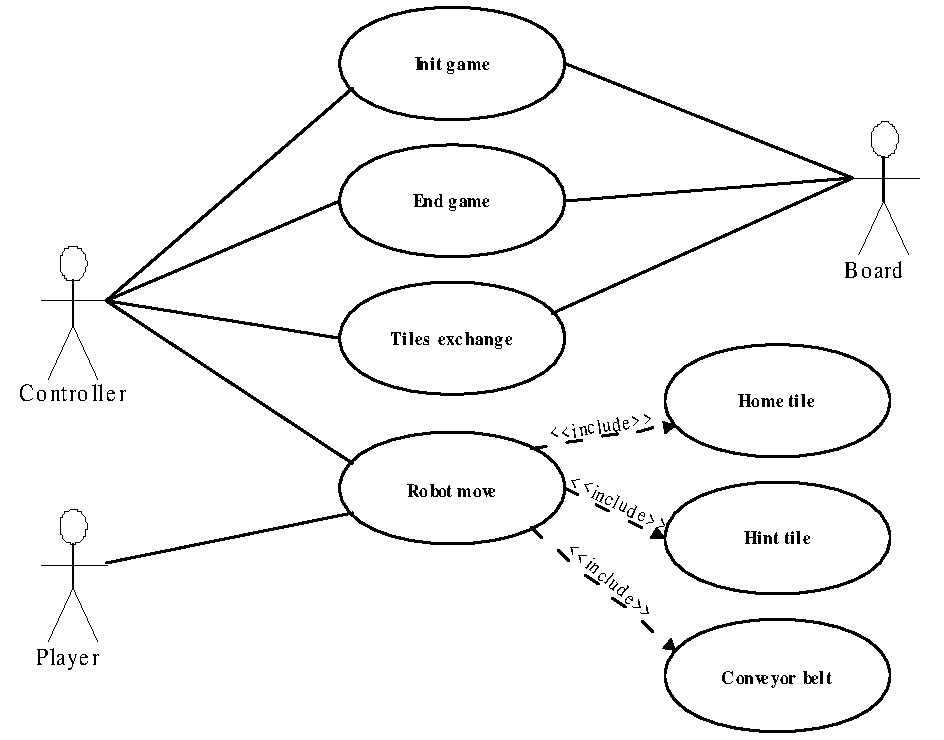
\includegraphics[width=\linewidth]{usecases/diagram.pdf}	

\subsection{High Level Message Sequence Chart}
	The following graph represents our high level message sequence chart and shows how a normal program flow is modeled by MSCs. The graph consists of two parts that run concurrently, the viewer part and the main game part. The viewer part will make sure the viewer updates regularly. The main game part follows the flow of a normal game.
	
	\digraph[scale=0.4]{HMSC}{
begin2 [label="",shape="invtriangle"];
end2 [label="",shape="triangle"];
initview [label="Initialize viewer",shape="Mrecord"];
updateview [label="Update viewer",shape="Mrecord"];
begin2->initview;
initview->updateview;
updateview->updateview;
updateview->end2;
begin [label="",shape="invtriangle"];
end [label="",shape="triangle"];
p1 [label="",shape="point"];
p2 [label="",shape="point"];
p22 [label="",shape="point"];
p3 [label="",shape="point"];
p4 [label="",shape="point"];
p5 [label="",shape="point"];
p55 [label="",shape="point"];
p6 [label="",shape="point"];
p66 [label="",shape="point"];
p7 [label="",shape="point"];
p77 [label="",shape="point"];
p8 [label="",shape="point"];
init [label="Initialize",shape="Mrecord"];
mvreq [label="Robot move request",shape="Mrecord"];
mvrej [label="Reject move",shape="Mrecord"];
retnt [label="Return Normal tile",shape="Mrecord"];
retht [label="Return Hint tile",shape="Mrecord"];
retct [label="Return Conveyor tile",shape="Mrecord"];
retmt [label="Return Home tile",shape="Mrecord"];
ordex [label="Ordinary exchange",shape="Mrecord"];
spcex [label="Special exchange",shape="Mrecord"];
endgame [label="End game",shape="Mrecord"];
notrob1 [label="Notify robots",shape="Mrecord"];
notrob2 [label="Notify robots",shape="Mrecord"];
begin->p1;
p1->init;
init->p2;
p2->mvreq;
mvreq->p3;
p3->mvrej;
mvrej->p2;
p3->p4;
p4->retnt;
p4->retht;
p4->retct;
p4->retmt;
retnt->p5;
retht->p5;
retct->p5;
p5->p55;
p55->p66;
p66->p6;
p55->notrob1;
notrob1->p66;
p6->ordex;
p6->spcex;
ordex->p7;
spcex->p7;
p7->p77;
p77->p22;
p22->p2 [tailport=e];
p77->notrob2;
notrob2->p22;
retmt->endgame;
endgame->p8;
p8->p1;
p8->end;
}

	%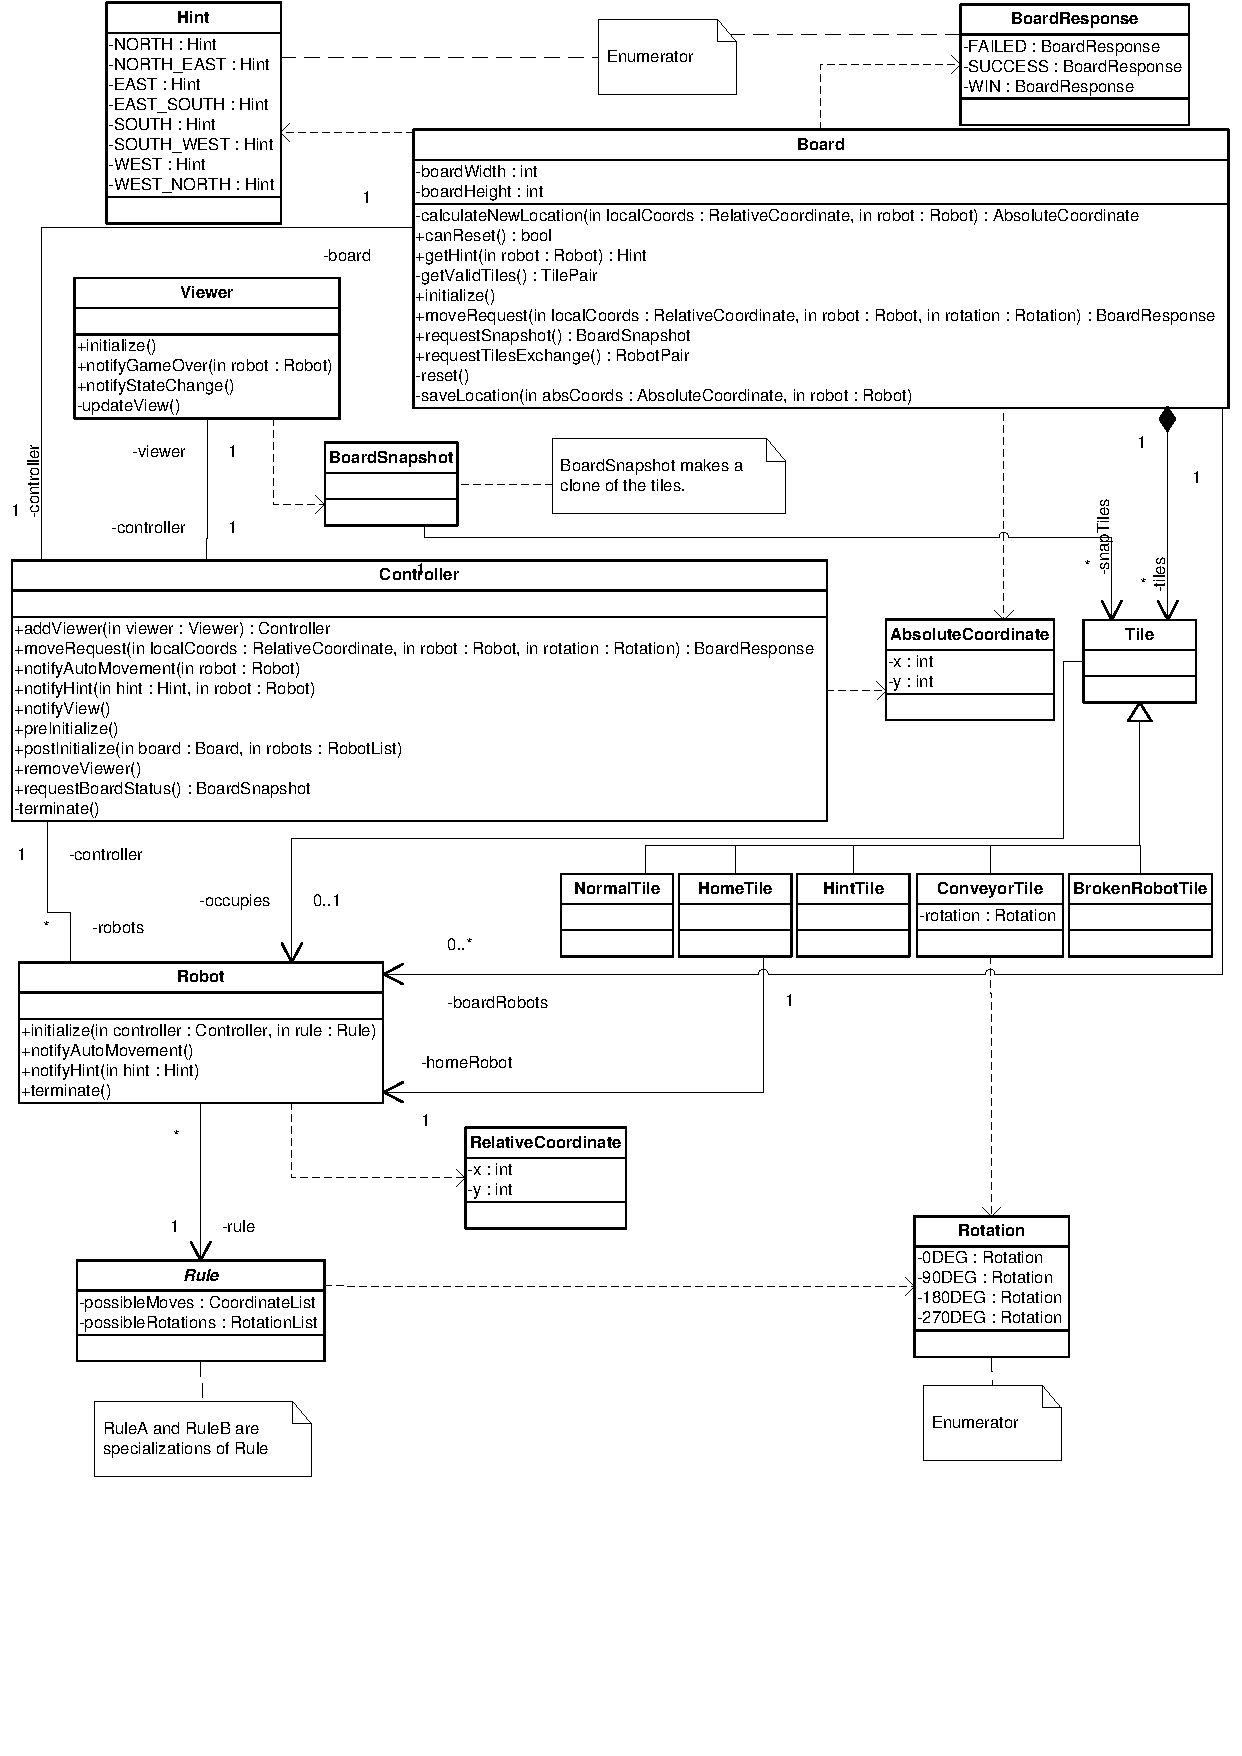
\includegraphics[width=\linewidth]{classdiagram}

\subsection{Message Sequence Charts}
	This section contains the message sequence charts for our use cases. Below every MSC is the location of the MSC in the High Level Message Sequence Chart.

	The world entity is not a real part of our MSCs, but rather a link to the outside world. When an internal action ends in '()' it's a function call to a private function of the entity. Otherwise, it's an action within the called function.

	We are using the following MSC syntax:

	\begin{msc}
	msc{
        	a, b;

        	a -> b [label="A signal"];
        	a => b [label="A function call"];
        	b >> a [label="A return value"];
        	b rbox b [label="An internal action"];

	}
\end{msc}


	Note: the symbol $\vdots$ denotes the start and end of a co-region.

	\subsubsection{Initialize viewer}
	The viewer is initialized by the world. Analogous to the HMSC, this happens concurrently to the Initialize MSC.
	
	\begin{msc}
msc
{

w [label="World"],
b [label="Board"],
c [label="Controller"],
v [label="Viewer"];

v box v [label=""],
b box b [label=""],
c box c [label=""],
w box w [label=""];

|||;

w => v [label="initialize(controller)"];
v rbox v [label="initialize"];
v => c [label="addViewer(viewer)"];
c >> v [label="self"];

... [label="board waits a predefined time"];

b rbox b [label="make snapshot"];
b -> c [label="notifyViewer(snapshot)"];
c -> v [label="notifyStateChange(snapshot)"];
v rbox v [label="updateView()"];

|||;

v box v [label="", textbgcolor="black"],
b box b [label="", textbgcolor="black"],
c box c [label="", textbgcolor="black"],
w box w [label="", textbgcolor="black"];

}
\end{msc}
\digraph[scale=0.5]{HMSC_init_view}{rankdir=LR;
p2 [label="",shape="point"];
init [label="Initialize",shape="Mrecord"];
initview [label="Initialize viewer",shape="Mrecord",style=filled];
mvreq [label="Robot move request",shape="Mrecord"];
init->initview;
initview->p2;
p2->mvreq
}


    	\subsubsection{Update viewer}
	During the game execution, the viewer will keep requesting the current board snapshot from the controller. This happens concurrently to the rest of the process. It can also request the board snapshot when it gets notified by the controller that the board has changed.
    	
	\begin{msc}
msc {

b [label="Board"],
c [label="Controller"],
d [label="Viewer"];

b box b [label=""],
d box d [label=""],
c box c [label=""];

|||;

d => c [label="requestBoardSnapshot()"];
c => b [label="requestBoardStatus()"];
b >> c [label="BoardSnapshot"];
c >> d [label="BoardSnapshot"];
d box d [label="updateView()"];

|||;

d box d [label="", textbgcolor="black"],
c box c [label="", textbgcolor="black"],
b box b [label="", textbgcolor="black"];

}
\end{msc}
\digraph[scale=0.5]{HMSC_upview}{
rankdir=LR;
end2 [label="",shape="triangle"];
initview [label="Initialize viewer",shape="Mrecord"];
updateview [label="Update viewer",shape="Mrecord",style=filled];
initview->updateview;
updateview->updateview;
updateview->end2;
} 

	\subsubsection{Initialize}
	When the game starts, the board is initialized. When this is done, the board sends a preInitialize to the controller. When the controller is done with that, the board will initialize all robots (choosing the appropriate rule for them), which will reply with an 'OK' when done. When all robots have been initialized, the board sends a postInitialize to the controller. All entities are now initialized. \\
	We introduced a separate pre- and post-initialize method, because the controller can not fully initialize without the robots and the robots, in turn, must be initialized with the controller. So, the pre-initialize is used to create the controller and the post-initialize is used to store all the robots that have been initialized by the board.
  	
	\begin{msc}
msc
{

a [label="Robot"],
b [label="Controller"],
c [label="Board"];

a box a [label=""],
b box b [label=""],
c box c [label=""];

|||;

b rbox b [label="initialize"];

b => a [label="initialize"];
a rbox a [label="initialize"];
a >> b [label=""];

b =>c [label="initialize(robotlist)"];
c rbox c [label="initliaze"];
c >>b [label="OK"];

|||;

a box a [label="", textbgcolor="black"],
b box b [label="", textbgcolor="black"],
c box c [label="", textbgcolor="black"];

}
\end{msc}
\digraph[scale=0.5]{HMSC_init}{rankdir=LR;
begin [label="",shape="invtriangle"];
p1 [label="",shape="point"];
p2 [label="",shape="point"];
init [label="Initialize",shape="Mrecord",style=filled];
mvreq [label="Robot move request",shape="Mrecord"];
begin->p1;
p1->init;
init->p2;
p2->mvreq
}

    	
	\subsubsection{Robot move request}
	A robot can make a move request with the controller, which will forward that to the board. The board will check the validity of the move itself with the robots rule and then check the validity of the move at the current state of the board.

	\begin{msc}
msc
{

d [label="Board"],
c [label="Controller"],
a [label="Robot"],
r [label="Rule"];

d box d [label=""],
c box c [label=""],
a box a [label=""],
r box r [label=""];

|||;

a => c [label="moveRequest(localCoords, robot, rotation)"];
c => d [label="moveRequest(localCoords, robot, rotation)"];
d rbox d [label="get possible moves"], r note r [label="references the robot's ruleset"];
d rbox d [label="get possible rotations"];
d rbox d [label="check if robot can be placed"];

|||;

a box a [label="", textbgcolor="black"],
c box c [label="", textbgcolor="black"],
d box d [label="", textbgcolor="black"],
r box r [label="", textbgcolor="black"];

}
\end{msc}
\digraph[scale=0.5]{HMSC_req}{
rankdir=LR;
p2 [label="",shape="point"];
p3 [label="",shape="point"];
p4 [label="",shape="point"];
init [label="Initialize",shape="Mrecord"];
mvreq [label="Robot move request",shape="Mrecord",style=filled];
mvrej [label="Reject move",shape="Mrecord"];
retnt [label="Return Normal tile",shape="Mrecord"];
retht [label="Return Hint tile",shape="Mrecord"];
retct [label="Return Conveyor tile",shape="Mrecord"];
retmt [label="Return Home tile",shape="Mrecord"];
init->p2;
p2->mvreq;
mvreq->p3;
p3->mvrej;
mvrej->p2;
p3->p4;
p4->retnt;
p4->retht;
p4->retct;
p4->retmt;
}


	\subsubsection{Return Normal tile}
	If the move request is okay, and the robot is moved to a normal tile, the board will return \emph{SUCCESS} to the controller, which will forward this message to the robot that was moved and then notify the viewer that the state of the board has changed.

	\begin{msc}
msc
{

d [label="Board"],
c [label="Controller"],
a [label="Robot"];

d box d [label=""],
c box c [label=""],
a box a [label=""];

|||;

d rbox d [label="calculateNewLocation(localCoords, robot)"];
d rbox d [label="saveLocation(absCoords, robot)"];
d >> c [label="SUCCESS"];
c >> a [label="SUCCESS"];

|||;

a box a [label="", textbgcolor="black"],
c box c [label="", textbgcolor="black"],
d box d [label="", textbgcolor="black"];

}
\end{msc}
\digraph[scale=0.5]{HMSC_mvnt}{
rankdir=LR;
p3 [label="",shape="point"];
p4 [label="",shape="point"];
p5 [label="",shape="point"];
p6 [label="",shape="point"];
notrob1 [label="Notify robots",shape="Mrecord"];
p55 [label="",shape="point"];
p66 [label="",shape="point"];
mvreq [label="Robot move request",shape="Mrecord"];
mvrej [label="Reject move",shape="Mrecord"];
retnt [label="Return Normal tile",shape="Mrecord",style=filled];
ordex [label="Ordinary exchange",shape="Mrecord"];
spcex [label="Special exchange",shape="Mrecord"];
mvreq->p3;
p3->mvrej;
p3->p4;
p4->retnt;
retnt->p5;
p5->p55;
p55->p66;
p66->p6;
p55->notrob1;
notrob1->p66;
p6->ordex;
p6->spcex;
}


	\subsubsection{Return Hint tile}
	If the move request is okay, and the robot is moved to a hint tile, the board will notify the controller that the robot that moved should receive a hint. The controller will notify the viewer that the state of the board has changed and forward the hint to the robot.

	\begin{msc}
msc
{

d [label="Board"],
c [label="Controller"],
a [label="Robot"];

d box d [label=""],
c box c [label=""],
a box a [label=""];

|||;

d rbox d [label="calculateNewLocation(localCoords, robot)"];
d rbox d [label="saveLocation(absCoords, robot)"];
d >> c [label="HINT"];
c => d [label="getHint(robot)"];
d rbox d [label="generate hint"];
d >> c [label="hint"];
c => a [label="notifyHint(hint)"];

|||;

a box a [label="", textbgcolor="black"],
c box c [label="", textbgcolor="black"],
d box d [label="", textbgcolor="black"];

}
\end{msc}
\digraph[scale=0.5]{HMSC_mvht}{
rankdir=LR;
p3 [label="",shape="point"];
p4 [label="",shape="point"];
p5 [label="",shape="point"];
p6 [label="",shape="point"];
mvreq [label="Robot move request",shape="Mrecord"];
mvrej [label="Reject move",shape="Mrecord"];
retht [label="Return Hint tile",shape="Mrecord",style=filled];
ordex [label="Ordinary exchange",shape="Mrecord"];
spcex [label="Special exchange",shape="Mrecord"];
mvreq->p3;
p3->mvrej;
p3->p4;
p4->retht;
retht->p5;
p5->p6;
p6->ordex;
p6->spcex;
}


	\subsubsection{Return Conveyor tile}
	If the move request is okay, and the robot is moved to a conveyor tile, the board will notify the controller that the robot was moved successfully. The controller will notify the viewer that the state of the board is updated and forward the message from the board to the robot. The board will then send a message to the controller that the robot was moved automatically (this was due to the conveyor belt) and the controller will forward this message to the robot.

	\begin{msc}
msc
{

d [label="Board"],
c [label="Controller"],
a [label="Robot"];

d box d [label=""],
c box c [label=""],
a box a [label=""];

|||;

d rbox d [label="calculateNewLocation(localCoords, robot)"];
d rbox d [label="saveLocation(absCoords, robot)"];
d >> c [label="SUCCESS"];
c >> a [label="SUCCESS"];

|||;

d -> c [label="notifyAutoMovement(robot)"];
c -> a [label="notifyAutoMovement()"];


|||;

a box a [label="", textbgcolor="black"],
c box c [label="", textbgcolor="black"],
d box d [label="", textbgcolor="black"];

}
\end{msc}
\digraph[scale=0.5]{HMSC_mvct}{
rankdir=LR;
p3 [label="",shape="point"];
p4 [label="",shape="point"];
p5 [label="",shape="point"];
p6 [label="",shape="point"];
notrob1 [label="Notify robots",shape="Mrecord"];
p55 [label="",shape="point"];
p66 [label="",shape="point"];
mvreq [label="Robot move request",shape="Mrecord"];
mvrej [label="Reject move",shape="Mrecord"];
retct [label="Return Conveyor tile",shape="Mrecord",style=filled];
ordex [label="Ordinary exchange",shape="Mrecord"];
spcex [label="Special exchange",shape="Mrecord"];
mvreq->p3;
p3->mvrej;
p3->p4;
p4->retct;
retct->p5;
p5->p55;
p55->p66;
p66->p6;
p55->notrob1;
notrob1->p66;
p6->ordex;
p6->spcex;
}


	\subsubsection{Return Home tile}
	If the move request is okay, and the robot is moved to its home tile, the board will notify the controller that the robot that moved wins the game. The controller notifies the viewer that the state of the board has changed.

	\begin{msc}
msc
{

a [label="Robot"],
c [label="Controller"],
d [label="Board"];

a box a [label=""],
c box c [label=""],
d box d [label=""];

|||;

d rbox d [label="calculateNewLocation(localCoords, robot)"];
d rbox d [label="saveLocation(absCoords, robot)"];
d >> c [label="WIN"];
c => a [label="terminate"];
a note a [label="each robot, except the robot that won the game, receives a terminate from the controller"];

|||;

a box a [label="", textbgcolor="black"],
c box c [label="", textbgcolor="black"],
d box d [label="", textbgcolor="black"];

}
\end{msc}



	\subsubsection{Reject move}
	If the move request is, for whatever reason, not okay, the board will notify the controller of this. The controller will forward this to the robot that tried to move.

	\begin{msc}
msc
{

a [label="Robot"],
c [label="Controller"],
d [label="Board"],
r [label="Rule"];

a box a [label=""],
c box c [label=""],
d box d [label=""],
r box r [label=""];

|||;

r >> d [label="NOK"];
d >> c [label="NOK"];
c -> a [label="NOK"];

|||;

a box a [label="", textbgcolor="black"],
c box c [label="", textbgcolor="black"],
d box d [label="", textbgcolor="black"],
r box r [label="", textbgcolor="black"];

}
\end{msc}
\digraph[scale=0.5]{HMSC_mvrej}{
rankdir=LR;
p2 [label="",shape="point"];
p3 [label="",shape="point"];
init [label="Initialize",shape="Mrecord"];
mvreq [label="Robot move request",shape="Mrecord"];
mvrej [label="Reject move",shape="Mrecord",style=filled];
init->p2;
p2->mvreq;
mvreq->p3;
p3->mvrej;
mvrej->p2;
}



	\advance\count17 by -6

	\subsubsection{Ordinary exchange}
	The controller requests the board to do a tile exchange. The board will get two valid tiles (internally, this function relies on the rule entities), swap them and returns an empty RobotPair to signal that there were no robots on the tiles.

	\begin{msc}
msc
{

b [label="Board"],
c [label="Controller"];

c box c [label=""],
b box b [label=""];

|||;

c=>b [label="requestTilesExchange()"];
b rbox b [label="exchange two tiles"];
b>>c [label="empty RobotPair"];

|||;

b box b [label="",textbgcolor="black"],
c box c [label="",textbgcolor="black"];

}
\end{msc}
\digraph[scale=0.5]{HMSC_exch}{
rankdir=LR;
p2 [label="",shape="point"];
p5 [label="",shape="point"];
p6 [label="",shape="point"];
p7 [label="",shape="point"];
init [label="Initialize",shape="Mrecord"];
mvreq [label="Robot move request",shape="Mrecord"];
retnt [label="Return Normal tile",shape="Mrecord"];
retht [label="Return Hint tile",shape="Mrecord"];
retct [label="Return Conveyor tile",shape="Mrecord"];
ordex [label="Ordinary exchange",shape="Mrecord",style=filled];
init->p2;
p2->mvreq;
retnt->p5;
retht->p5;
retct->p5;
p5->p6;
p6->ordex;
ordex->p7;
p7->p2;
}


	\subsubsection{Special exchange}
	Like in the ordinary exchange, the controller requests the board to do a tile exchange. The board will find two valid tiles (with on at least one of them a robot or a conveyor belt) and swap them. The board will return a RobotPair with the robots that have been selected in it (so either an empty RobotPair, a RobotPair with one robot, or a RobotPair with two robots). The selected conveyor tiles and robots will be rotated. The controller will notify all players that have been moved and then notify the viewer that the state of the board has changed. Here, one robot and one conveyor belt have been selected.

	\begin{msc}
msc
{

b [label="Board"],
c [label="Controller"],
p1 [label="Robot1"],
p2 [label="Robot2"],
v [label="Viewer"];

c box c [label=""],
b box b [label=""],
p1 box p1 [label=""],
p2 box p2 [label=""],
v box v [label=""];

|||;
c=>b [label="requestTilesExchange()"];
b rbox b [label="getValidTiles()"];
b rbox b [label="exchange two valid tiles"];
b rbox b [label="rotate robot1 and rotate tiles"];
b>>c [label="RobotPair with one robot"];
...;
c->p1 [label="notifyAutoMovement()"];
c -> v [label="notifyStateChange()"];
...;

|||;

b box b [label="",textbgcolor="black"],
c box c [label="",textbgcolor="black"],
p1 box p1 [label="",textbgcolor="black"],
p2 box p2 [label="",textbgcolor="black"],
v box v [label="",textbgcolor="black"];

}
\end{msc}

\digraph[scale=0.5]{HMSC_exchsp}{
rankdir=LR;
p2 [label="",shape="point"];
p5 [label="",shape="point"];
p6 [label="",shape="point"];
p7 [label="",shape="point"];
p22 [label="",shape="point"];
p77 [label="",shape="point"];
notrob2 [label="Notify robots",shape="Mrecord"];
init [label="Initialize",shape="Mrecord"];
mvreq [label="Robot move request",shape="Mrecord"];
retnt [label="Return Normal tile",shape="Mrecord"];
retht [label="Return Hint tile",shape="Mrecord"];
retct [label="Return Conveyor tile",shape="Mrecord"];
spcex [label="Special exchange",shape="Mrecord",style=filled];
init->p2;
p2->mvreq;
retnt->p5;
retht->p5;
retct->p5;
p5->p6;
p6->spcex;
spcex->p7;
p7->p77;
p77->p22;
p22->p2;
p77->notrob2;
notrob2->p22;
}

	
	\subsubsection{Notify robots}
	The board sends a notification to the controller, which forwards this to the robot that was moved. This MSC is used when a robot is moved due to the move of another robot, for example when a robot that blocked the end of a conveyor belt moves away and the last robot on the belt should move to the end.

	The notify robots MSC will be inserted here.


	\subsubsection{End game}
	The controller will send a terminate message to all losing robots, which will then terminate safely. The controller will then notify the viewer which robot won the game, so it can show the end game animation. When the animation is done, the call will return and the controller will send a message to the board that everything it done and the board can reset and will then terminate. The winning robot will also terminate. The board can then choose to either reset to start a new game or terminate.

	\begin{msc}
msc
{

b [label="Board"],
c [label="Controller"],
p [label="Robot"],
v [label="View"];

b box b [label=""],
c box c [label=""],
p box p [label=""],
v box v [label=""];

|||;

c -> p [label="terminate"];
p rbox p [label="terminate()"];
p note p [label="From here on, robot is the robot that has won the game"];
c -> v [label="notifyGameOver(robot)"];
v rbox v [label="fireworks"];
v >> c [label="done"];
c -> b [label="canReset"];
v rbox v [label="terminate"],
b rbox b [label="reset()"],
c rbox c [label="terminate()"];


|||;

b box b [label="",textbgcolor="black"],
c box c [label="",textbgcolor="black"],
p box p [label="",textbgcolor="black"],
v box v [label="",textbgcolor="black"];

}
\end{msc}
\digraph[scale=0.5]{HMSC_end}{
rankdir=LR;
begin [label="",shape="invtriangle"];
end [label="",shape="triangle"];
p1 [label="",shape="point"];
p8 [label="",shape="point"];
init [label="Initialize",shape="Mrecord"];
retmt [label="Return Home tile",shape="Mrecord"];
endgame [label="End game",shape="Mrecord",style=filled];
begin->p1;
p1->init;
retmt->endgame;
endgame->p8;
p8->p1;
p8->end;
}

